\documentclass{standalone}
\usepackage{tikz}
\usetikzlibrary{patterns, positioning}

\begin{document}
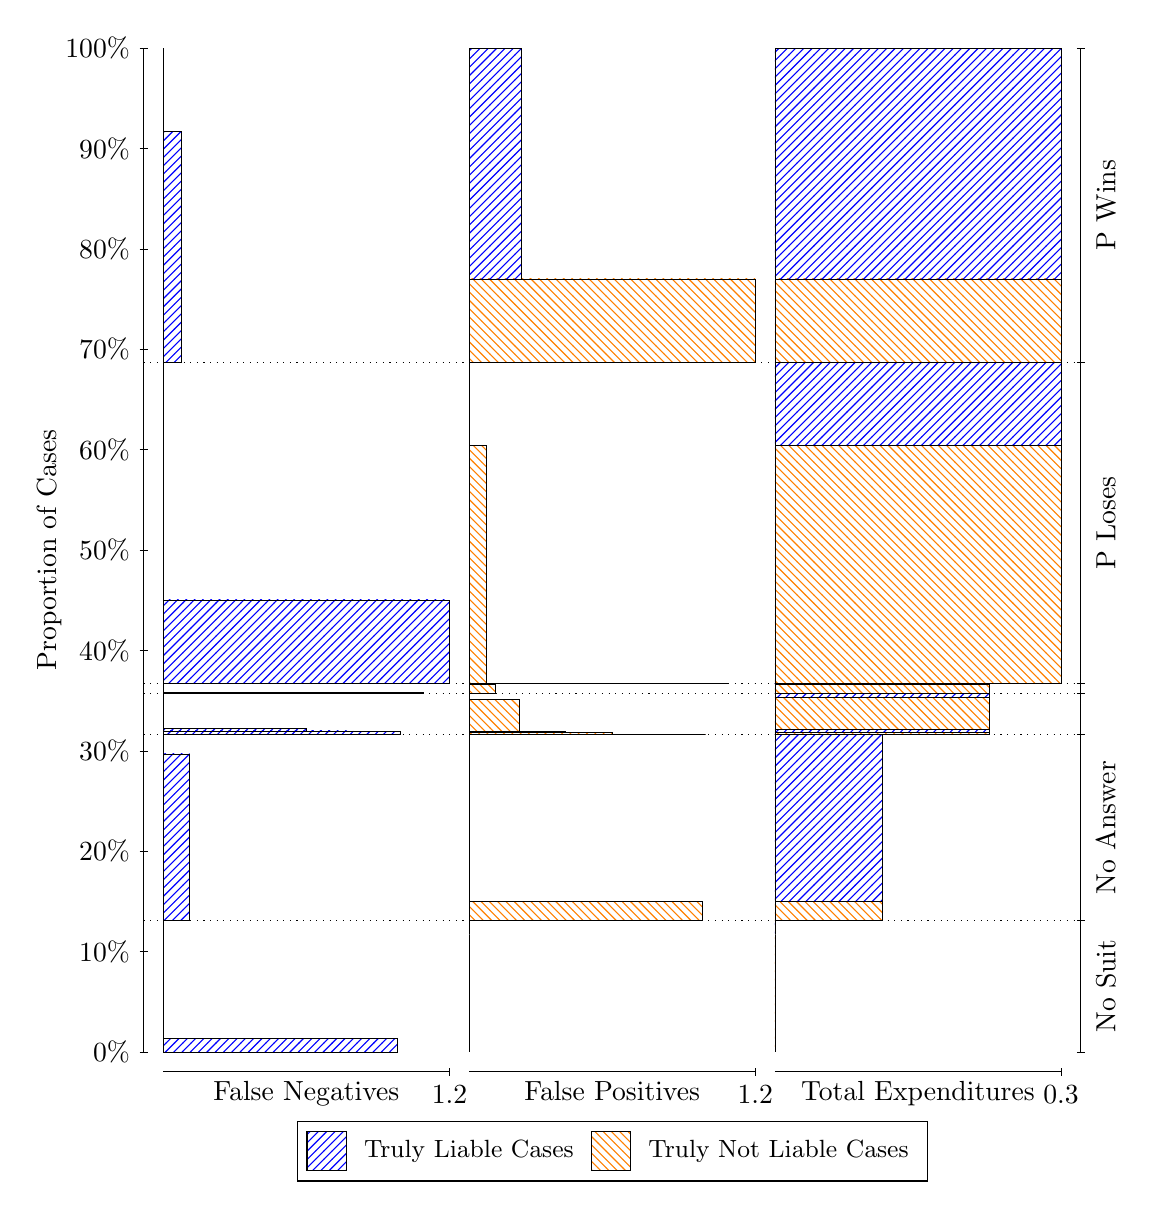
\begin{tikzpicture}
\draw[black, very thin] (1.5,1.75) -- (1.5,14.5);
\node[rotate=90, anchor=center] at (0.3, 8.125) {Proportion of Cases};
\draw[black, very thin] (1.45,1.75) -- (1.55,1.75);
\node[anchor=east] at (1.45, 1.75) {0\%};
\draw[black, very thin] (1.45,3.025) -- (1.55,3.025);
\node[anchor=east] at (1.45, 3.025) {10\%};
\draw[black, very thin] (1.45,4.3) -- (1.55,4.3);
\node[anchor=east] at (1.45, 4.3) {20\%};
\draw[black, very thin] (1.45,5.575) -- (1.55,5.575);
\node[anchor=east] at (1.45, 5.575) {30\%};
\draw[black, very thin] (1.45,6.85) -- (1.55,6.85);
\node[anchor=east] at (1.45, 6.85) {40\%};
\draw[black, very thin] (1.45,8.125) -- (1.55,8.125);
\node[anchor=east] at (1.45, 8.125) {50\%};
\draw[black, very thin] (1.45,9.4) -- (1.55,9.4);
\node[anchor=east] at (1.45, 9.4) {60\%};
\draw[black, very thin] (1.45,10.675) -- (1.55,10.675);
\node[anchor=east] at (1.45, 10.675) {70\%};
\draw[black, very thin] (1.45,11.95) -- (1.55,11.95);
\node[anchor=east] at (1.45, 11.95) {80\%};
\draw[black, very thin] (1.45,13.225) -- (1.55,13.225);
\node[anchor=east] at (1.45, 13.225) {90\%};
\draw[black, very thin] (1.45,14.5) -- (1.55,14.5);
\node[anchor=east] at (1.45, 14.5) {100\%};

\draw[black, very thin] (13.4,1.75) -- (13.4,14.5);
\draw[black, very thin] (13.35,1.75) -- (13.45,1.75);
\node[anchor=west] at (13.35, 1.75) {};
\draw[black, very thin] (13.35,3.4205) -- (13.45,3.4205);
\node[anchor=west] at (13.35, 3.4205) {};
\draw[black, very thin] (13.35,5.7807) -- (13.45,5.7807);
\node[anchor=west] at (13.35, 5.7807) {};
\draw[black, very thin] (13.35,6.303) -- (13.45,6.303);
\node[anchor=west] at (13.35, 6.303) {};
\draw[black, very thin] (13.35,6.4325) -- (13.45,6.4325);
\node[anchor=west] at (13.35, 6.4325) {};
\draw[black, very thin] (13.35,6.4325) -- (13.45,6.4325);
\node[anchor=west] at (13.35, 6.4325) {};
\draw[black, very thin] (13.35,10.509) -- (13.45,10.509);
\node[anchor=west] at (13.35, 10.509) {};
\draw[black, very thin] (13.35,14.5) -- (13.45,14.5);
\node[anchor=west] at (13.35, 14.5) {};

\draw[black, very thin, pattern color=blue, pattern=north east lines] (1.75,1.75) rectangle (4.716,1.9258);
\draw[black, very thin, pattern color=orange, pattern=north west lines] (1.75,1.9258) rectangle (1.75,3.4205);
\draw[black, very thin, pattern color=blue, pattern=north east lines] (1.75,3.4205) rectangle (2.0837,5.5371);
\draw[black, very thin, pattern color=orange, pattern=north west lines] (1.75,5.5371) rectangle (1.75,5.7807);
\draw[black, very thin, pattern color=blue, pattern=north east lines] (1.75,5.7807) rectangle (4.7531,5.8232);
\draw[black, very thin, pattern color=blue, pattern=north east lines] (1.75,5.8232) rectangle (4.4565,5.8253);
\draw[black, very thin, pattern color=blue, pattern=north east lines] (1.75,5.8253) rectangle (4.1599,5.8279);
\draw[black, very thin, pattern color=blue, pattern=north east lines] (1.75,5.8279) rectangle (3.8633,5.8279);
\draw[black, very thin, pattern color=blue, pattern=north east lines] (1.75,5.8279) rectangle (3.8633,5.8282);
\draw[black, very thin, pattern color=blue, pattern=north east lines] (1.75,5.8282) rectangle (3.5667,5.8588);
\draw[black, very thin, pattern color=blue, pattern=north east lines] (1.75,5.8588) rectangle (3.2701,5.8588);
\draw[black, very thin, pattern color=blue, pattern=north east lines] (1.75,5.8588) rectangle (2.9735,5.8588);
\draw[black, very thin, pattern color=blue, pattern=north east lines] (1.75,5.8588) rectangle (2.6769,5.8588);
\draw[black, very thin, pattern color=blue, pattern=north east lines] (1.75,5.8588) rectangle (2.3803,5.8588);
\draw[black, very thin, pattern color=orange, pattern=north west lines] (1.75,5.8588) rectangle (1.75,6.303);
\draw[black, very thin, pattern color=blue, pattern=north east lines] (1.75,6.303) rectangle (5.0497,6.3159);
\draw[black, very thin, pattern color=orange, pattern=north west lines] (1.75,6.3159) rectangle (1.75,6.4325);
\draw[black, very thin, pattern color=blue, pattern=north east lines] (1.75,6.4325) rectangle (2.0837,6.4325);
\draw[black, very thin, pattern color=orange, pattern=north west lines] (1.75,6.4325) rectangle (1.75,6.4325);
\draw[black, very thin, pattern color=blue, pattern=north east lines] (1.75,6.4325) rectangle (5.3833,7.4926);
\draw[black, very thin, pattern color=orange, pattern=north west lines] (1.75,7.4926) rectangle (1.75,10.509);
\draw[black, very thin, pattern color=blue, pattern=north east lines] (1.75,10.509) rectangle (1.9724,13.44);
\draw[black, very thin, pattern color=orange, pattern=north west lines] (1.75,13.44) rectangle (1.75,14.5);
\draw[black, very thin, pattern color=orange, pattern=north west lines] (5.6333,1.75) rectangle (5.6333,3.2448);
\draw[black, very thin, pattern color=blue, pattern=north east lines] (5.6333,3.2448) rectangle (5.6333,3.4205);
\draw[black, very thin, pattern color=orange, pattern=north west lines] (5.6333,3.4205) rectangle (8.5993,3.6641);
\draw[black, very thin, pattern color=blue, pattern=north east lines] (5.6333,3.6641) rectangle (5.6333,5.7807);
\draw[black, very thin, pattern color=orange, pattern=north west lines] (5.6333,5.7807) rectangle (8.6364,5.7807);
\draw[black, very thin, pattern color=orange, pattern=north west lines] (5.6333,5.7807) rectangle (8.3398,5.7807);
\draw[black, very thin, pattern color=orange, pattern=north west lines] (5.6333,5.7807) rectangle (8.0432,5.7807);
\draw[black, very thin, pattern color=orange, pattern=north west lines] (5.6333,5.7807) rectangle (7.7466,5.7807);
\draw[black, very thin, pattern color=orange, pattern=north west lines] (5.6333,5.7807) rectangle (7.45,5.8116);
\draw[black, very thin, pattern color=orange, pattern=north west lines] (5.6333,5.8116) rectangle (7.1534,5.8123);
\draw[black, very thin, pattern color=orange, pattern=north west lines] (5.6333,5.8123) rectangle (6.8568,5.8184);
\draw[black, very thin, pattern color=orange, pattern=north west lines] (5.6333,5.8184) rectangle (6.5602,5.8254);
\draw[black, very thin, pattern color=orange, pattern=north west lines] (5.6333,5.8254) rectangle (6.2636,6.2249);
\draw[black, very thin, pattern color=blue, pattern=north east lines] (5.6333,6.2249) rectangle (5.6704,6.2249);
\draw[black, very thin, pattern color=blue, pattern=north east lines] (5.6333,6.2249) rectangle (5.6333,6.303);
\draw[black, very thin, pattern color=orange, pattern=north west lines] (5.6333,6.303) rectangle (5.967,6.4195);
\draw[black, very thin, pattern color=blue, pattern=north east lines] (5.6333,6.4195) rectangle (5.6333,6.4325);
\draw[black, very thin, pattern color=orange, pattern=north west lines] (5.6333,6.4325) rectangle (8.933,6.4325);
\draw[black, very thin, pattern color=blue, pattern=north east lines] (5.6333,6.4325) rectangle (5.967,6.4325);
\draw[black, very thin, pattern color=orange, pattern=north west lines] (5.6333,6.4325) rectangle (5.8558,9.4489);
\draw[black, very thin, pattern color=blue, pattern=north east lines] (5.6333,9.4489) rectangle (5.6333,10.509);
\draw[black, very thin, pattern color=orange, pattern=north west lines] (5.6333,10.509) rectangle (9.2667,11.569);
\draw[black, very thin, pattern color=blue, pattern=north east lines] (5.6333,11.569) rectangle (6.3007,14.5);
\draw[black, very thin, pattern color=orange, pattern=north west lines] (9.5167,1.75) rectangle (9.5167,3.2448);
\draw[black, very thin, pattern color=blue, pattern=north east lines] (9.5167,3.2448) rectangle (9.5167,3.4205);
\draw[black, very thin, pattern color=orange, pattern=north west lines] (9.5167,3.4205) rectangle (10.879,3.6641);
\draw[black, very thin, pattern color=blue, pattern=north east lines] (9.5167,3.6641) rectangle (10.879,5.7807);
\draw[black, very thin, pattern color=orange, pattern=north west lines] (9.5167,5.7807) rectangle (12.242,5.7807);
\draw[black, very thin, pattern color=blue, pattern=north east lines] (9.5167,5.7807) rectangle (12.242,5.7807);
\draw[black, very thin, pattern color=orange, pattern=north west lines] (9.5167,5.7807) rectangle (12.242,5.8116);
\draw[black, very thin, pattern color=blue, pattern=north east lines] (9.5167,5.8116) rectangle (12.242,5.8422);
\draw[black, very thin, pattern color=orange, pattern=north west lines] (9.5167,5.8422) rectangle (12.242,6.2548);
\draw[black, very thin, pattern color=blue, pattern=north east lines] (9.5167,6.2548) rectangle (12.242,6.302);
\draw[black, very thin, pattern color=orange, pattern=north west lines] (9.5167,6.302) rectangle (12.242,6.3027);
\draw[black, very thin, pattern color=blue, pattern=north east lines] (9.5167,6.3027) rectangle (12.242,6.303);
\draw[black, very thin, pattern color=orange, pattern=north west lines] (9.5167,6.303) rectangle (12.242,6.303);
\draw[black, very thin, pattern color=blue, pattern=north east lines] (9.5167,6.303) rectangle (12.242,6.303);
\draw[black, very thin, pattern color=orange, pattern=north west lines] (9.5167,6.303) rectangle (12.242,6.4195);
\draw[black, very thin, pattern color=blue, pattern=north east lines] (9.5167,6.4195) rectangle (12.242,6.4325);
\draw[black, very thin, pattern color=orange, pattern=north west lines] (9.5167,6.4325) rectangle (12.242,6.4325);
\draw[black, very thin, pattern color=blue, pattern=north east lines] (9.5167,6.4325) rectangle (12.242,6.4325);
\draw[black, very thin, pattern color=orange, pattern=north west lines] (9.5167,6.4325) rectangle (13.15,9.4489);
\draw[black, very thin, pattern color=blue, pattern=north east lines] (9.5167,9.4489) rectangle (13.15,10.509);
\draw[black, very thin, pattern color=orange, pattern=north west lines] (9.5167,10.509) rectangle (13.15,11.569);
\draw[black, very thin, pattern color=blue, pattern=north east lines] (9.5167,11.569) rectangle (13.15,14.5);
\draw[black, dotted] (1.5,3.4205) -- (13.4,3.4205);
\draw[black, dotted] (1.5,5.7807) -- (13.4,5.7807);
\draw[black, dotted] (1.5,6.303) -- (13.4,6.303);
\draw[black, dotted] (1.5,6.4325) -- (13.4,6.4325);
\draw[black, dotted] (1.5,6.4325) -- (13.4,6.4325);
\draw[black, dotted] (1.5,10.509) -- (13.4,10.509);
\draw[black, very thin] (1.75,1.5) -- (5.3833,1.5);
\node[anchor=north] at (3.5667, 1.5) {False Negatives};
\draw[black, very thin] (5.3833,1.45) -- (5.3833,1.55);
\node[anchor=north] at (5.3833, 1.45) {1.2};

\draw[black, very thin] (5.6333,1.5) -- (9.2667,1.5);
\node[anchor=north] at (7.45, 1.5) {False Positives};
\draw[black, very thin] (9.2667,1.45) -- (9.2667,1.55);
\node[anchor=north] at (9.2667, 1.45) {1.2};

\draw[black, very thin] (9.5167,1.5) -- (13.15,1.5);
\node[anchor=north] at (11.333, 1.5) {Total Expenditures};
\draw[black, very thin] (13.15,1.45) -- (13.15,1.55);
\node[anchor=north] at (13.15, 1.45) {0.3};

\node[black, centered, rotate=90] at (13.72, 2.5853) {No Suit};
\node[black, centered, rotate=90] at (13.72, 4.6006) {No Answer};



\node[black, centered, rotate=90] at (13.72, 8.4707) {P Loses};
\node[black, centered, rotate=90] at (13.72, 12.504) {P Wins};

\draw (7.449999999999999,1.5) node[draw=none] (baseCoordinate) {};
\begin{scope}[align=center]
        \matrix[scale=0.5, draw=black, below=0.5cm of baseCoordinate, nodes={draw}, column sep=0.1cm]{
            \node[rectangle, draw, minimum width=0.5cm, minimum height=0.5cm, pattern=north east lines, pattern color=blue] {}; &
            \node[draw=none, font=\small] (B) {Truly Liable Cases}; &
            \node[rectangle, draw, minimum width=0.5cm, minimum height=0.5cm, pattern=north west lines, pattern color=orange] {}; &
            \node[draw=none, font=\small] (B) {Truly Not Liable Cases}; \\
            };
\end{scope}

\end{tikzpicture}
\end{document}